\documentclass{article}
\usepackage{tabularx,ragged2e,booktabs,caption}
\usepackage{graphicx}
\usepackage{float}
\usepackage{hyperref}
\usepackage{array}
\usepackage{graphicx}
\graphicspath{{imgs/}}
\usepackage{amsmath}
\usepackage{caption}
\usepackage{subcaption}
\usepackage{hyperref}
\usepackage[ruled,linesnumbered]{algorithm2e}
\usepackage{amssymb}
\usepackage{pgfplots}

\usepackage{tikz}
\usetikzlibrary{positioning,matrix, arrows.meta, patterns}

\newcommand{\kdtree}{\emph{k}-d tree}
\newcommand{\Mod}[1]{\ (\mathrm{mod}\ #1)}


\title{Implementation of a \kdtree{} using MPI and OpenMP}
\author{Francesco Andreuzzi}
\date{\today}

\begin{document}
\maketitle

\tableofcontents
\bibliographystyle{plain}

\section{Introduction} \label{sec:intro}
\kdtree{} is an established data structure which enables the use of a
plethora of efficient algorithms of huge practical interest, for instance
\emph{search algorithms} and \emph{nearest neighbor queries}
\cite{bentley1975multidimensional}. Another important aspect is the existence of
efficient utility algorithms which make quite efficient the update of the data
structure in response to changes in the dataset (deletion, insertion, \dots).

In this brief report we present and analyze a parallel implementations of
\kdtree{} which uses two standard frameworks for parallel programming, namely
OpenMP (shared memory) and MPI (distributed
memory). Our implementation uses the same approach for parallelization in
both cases, even though some compiler-level flags can be used to activate
different code regions whose goal is to fix performance bottlenecks peculiar of
a framework (for instance \emph{false-sharing} in OpenMP). We talk
briefly about this point below.

First things first: we briefly discuss the data structure and the invariants to
be maintained. Afterwards we present the very simple parallel algorithm we
developed, and spend a few words on the implementation. We then procede with
some considerations on our expectations for the performance, and verify our
hypothesis against the real data we extracted from a set of run of the code.

\section{\kdtree{}}
Given a set of k-dimensional points $P = \{p^1, \dots, p^n\}$ such that
$p^i \in \mathbb{R}^k$ we pick a recursive definition of a \kdtree{}
\cite{skrodzki2019kd}. The node of the tree associated with the set $P$ is given
by:
\begin{gather} \label{eq:recursive_kdtree_definition}
    \text{Node}(P) = \begin{cases}
        \text{null} &\text{if } P = \emptyset\\
        \{p_m, \text{Node}(P_1), \text{Node}(P_2)\} &\text{otherwise}
    \end{cases}
\end{gather}
where $p_m$ is the median point of $P$ against some axis $i$ which is chosen
via an unspecified criteria that we are going to formalize in some lines.
$P_1, P_2 \subset P$ are defined as follows:
\begin{gather*}
    P_1 = \{p \in P \mid p < p_m\} \qquad P_2 = \{p \in P \mid p > p_m\}
\end{gather*}
i.e. they are the subsets of points of $P$ which ``fall'' respectively before
and after $p_m$ along the i-th axis. For simplicity we assumed that $P$ does not
contain repeated values, however the definition is easily generalized.
$\text{Node}(P_1), \text{Node}(P_2)$ in (\ref*{eq:recursive_kdtree_definition})
are respectively the left and right branch which originate from
$\text{Node}(P)$.

The axis $i$ is chosen in such a way that the spread of the points in $P$ is
maximum along $i$. However, since we assumed that our points are distributed
somewhat uniformly in the space $\mathbb{R}^k$, we are going to use a very
simple function to determine the axis $i$ used to "split" the tree:
\begin{gather} \label{eq:axis_criteria}
    i(\ell) = \ell \Mod{k}
\end{gather}
where $\ell$ is the current level of the tree (i.e. the distance of the current
node from the root).

\begin{figure}[b!]
    \makebox[\textwidth][c]{
        \begin{subfigure}{.4\textwidth}
            \centering
            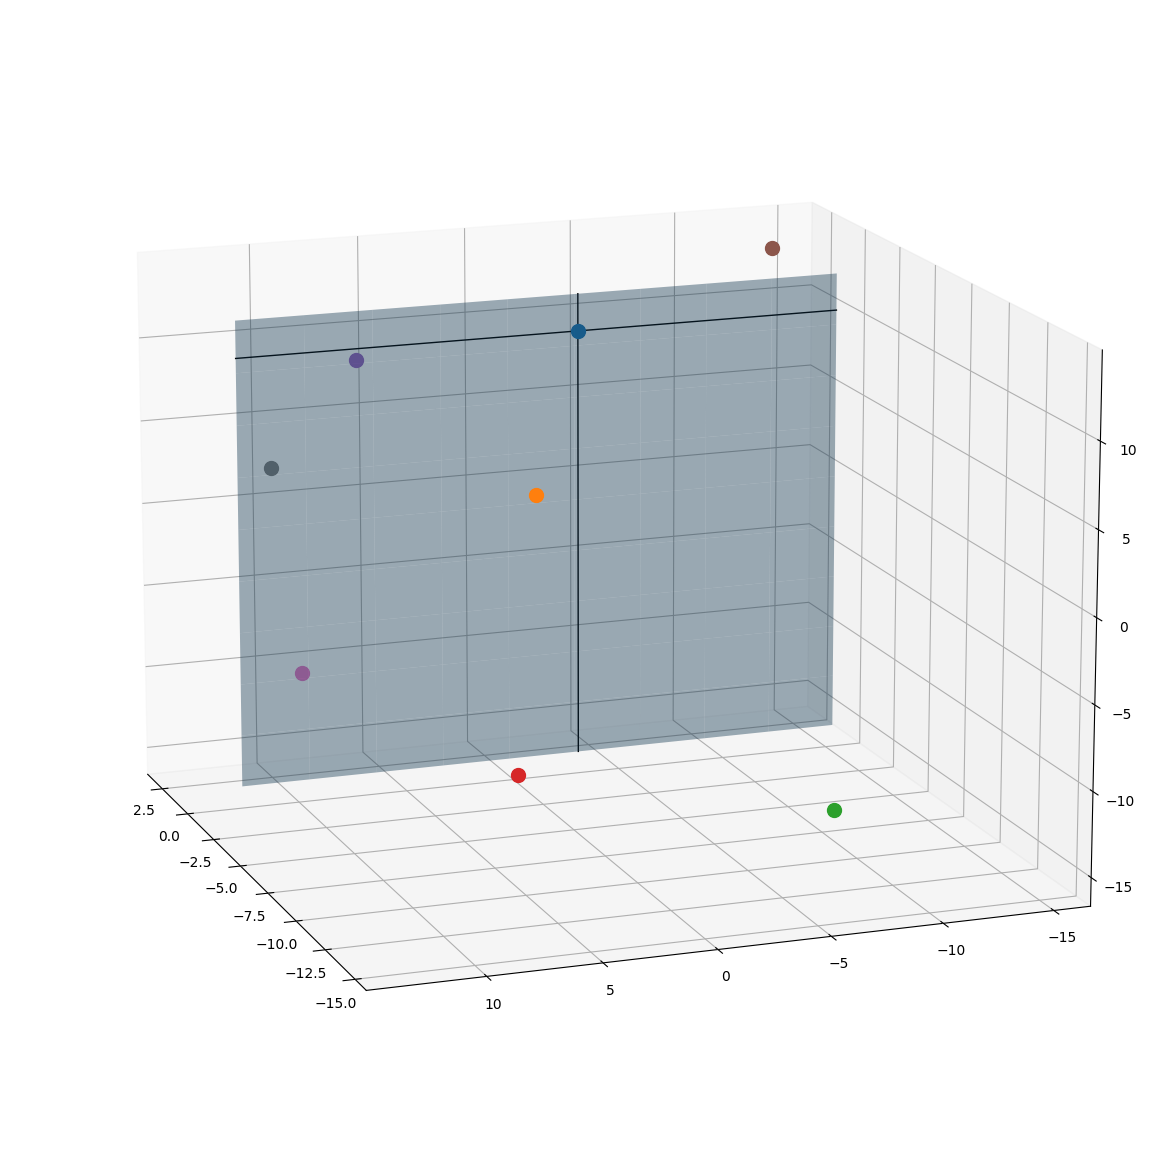
\includegraphics[width=\linewidth]{kd_tree_progress_img0.png}
            \caption{Depth 0}
        \end{subfigure}%
        \hfill
        \begin{subfigure}{.4\textwidth}
            \centering
            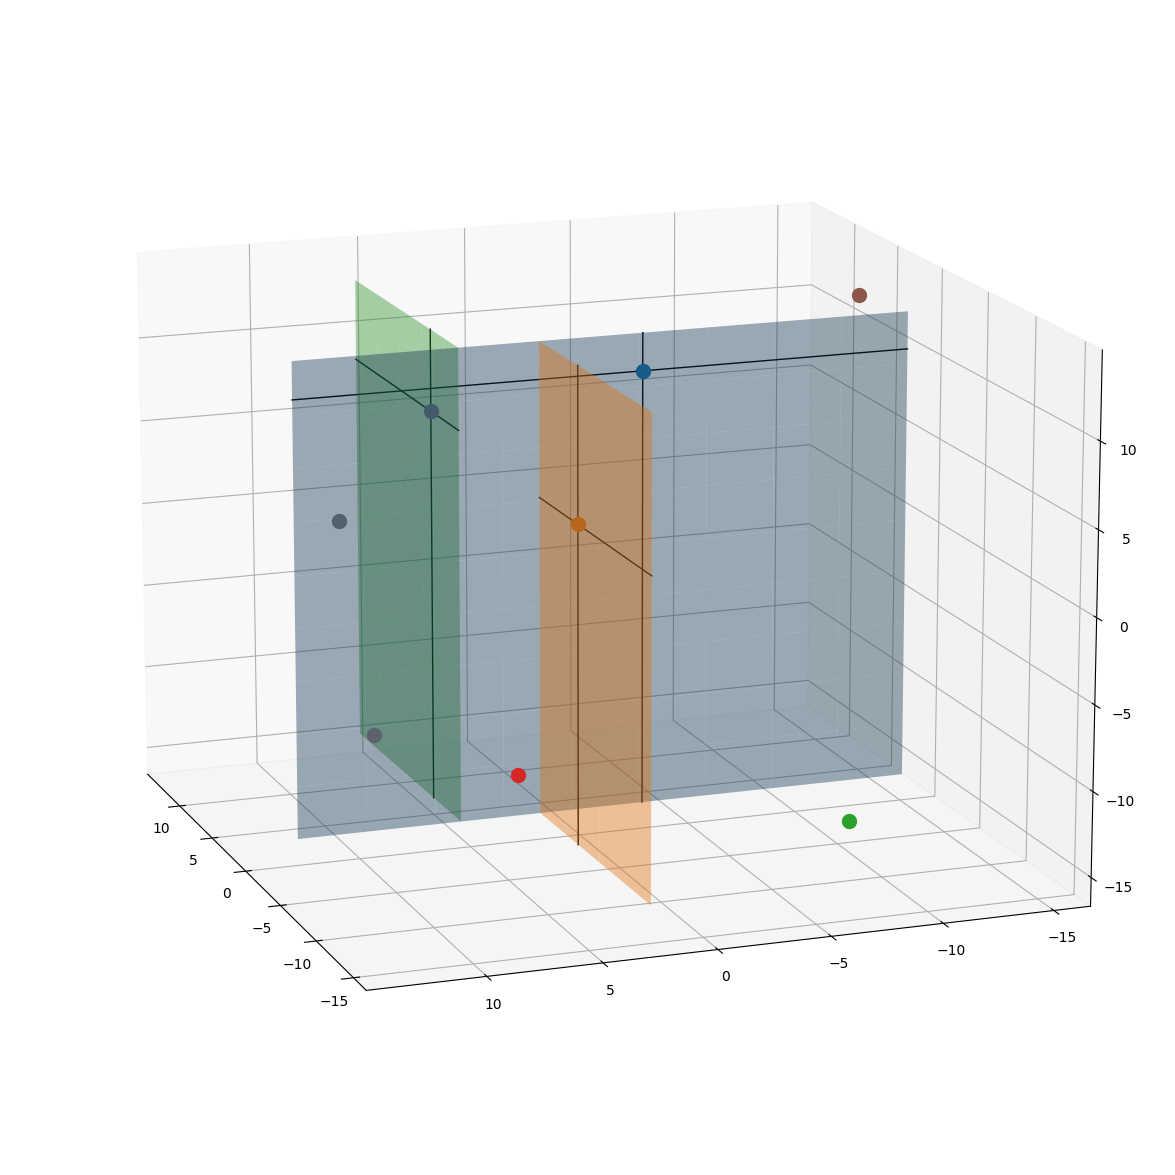
\includegraphics[width=\linewidth]{kd_tree_progress_img1.png}
            \caption{Depth 1}
        \end{subfigure}
        \hfill
        \begin{subfigure}{.4\textwidth}
            \centering
            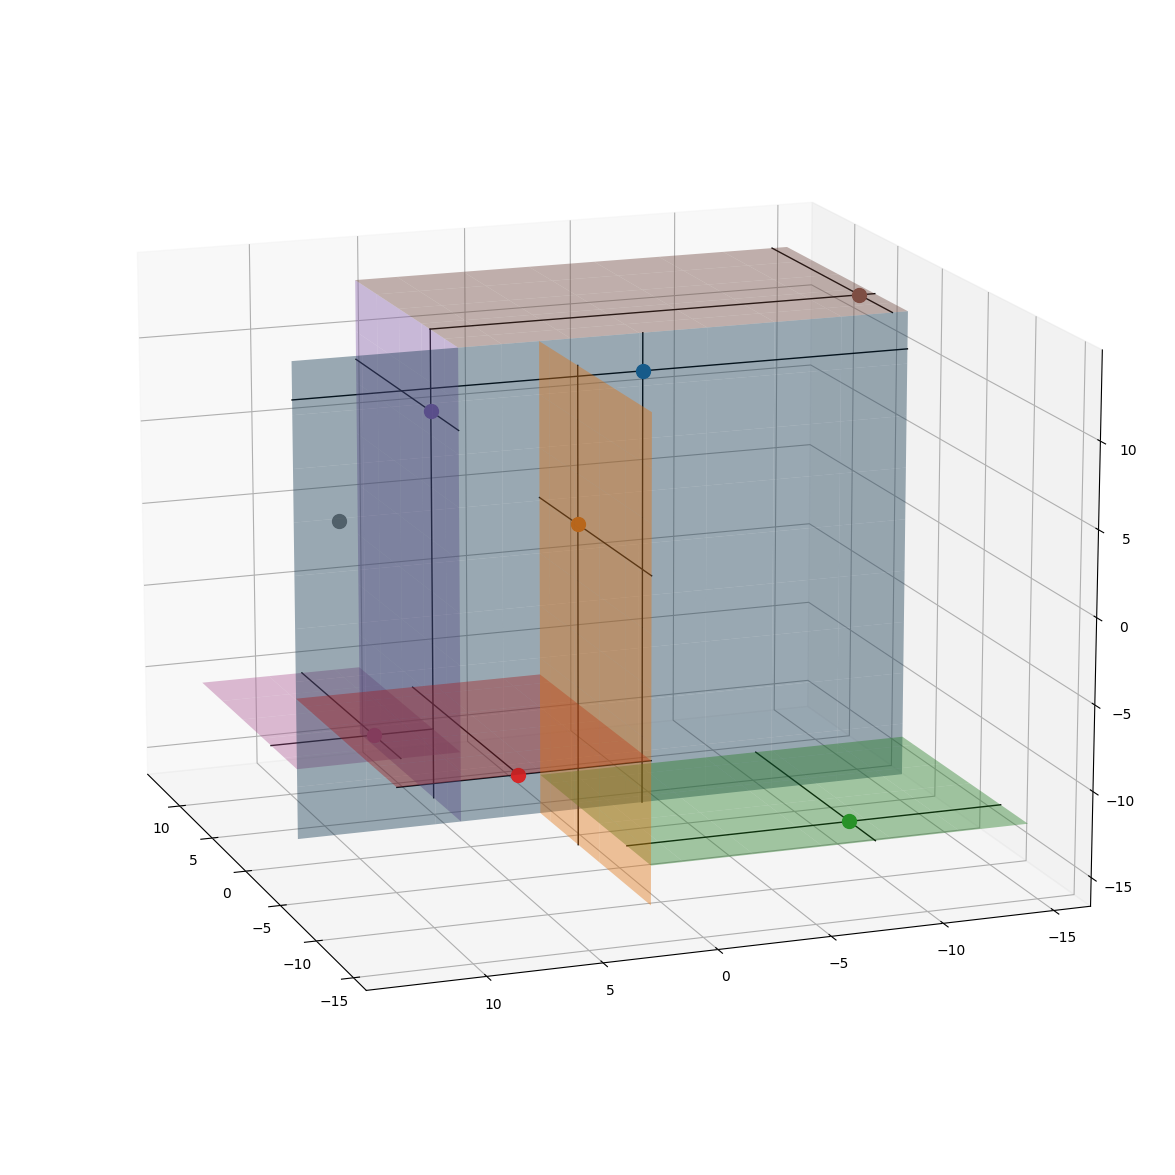
\includegraphics[width=\linewidth]{kd_tree_progress_img2.png}
            \caption{Depth 2}
        \end{subfigure}
    }
    \caption{A \kdtree{} (surfaces representation).}
    \label{fig:kdtree_surfaces_progression}
\end{figure}

Using a
\href{https://github.com/fAndreuzzi/parallel-kd-tree/tree/master/visualization}{visualizer tool}
written in Python which we developed for the occasion, we show the progression
of the construction of a \kdtree{} for a very simple dataset. The visualization
in Figure \ref{fig:kdtree_surfaces_progression} renders in a
very clear way the fact that points added to the tree in the level $k$ need to
satisfy constraints given by all the median points points in the parent branches
in levels $0, \dots, k-1$, against all the axes considered up to this level.
Each surface is the plane containing one of the points
added to the tree at some point of the algorithm, and divides the volume
dedicated to the corresponding branch in two halves which shall contain all the
other points (respectively) in the left and right branch. This is in a certain
sense a visual transposition of (\ref*{eq:recursive_kdtree_definition}).

However, in order to communicate the structure of the tree
the visualization shown in Figure \ref{fig:kdtree_branches_progression} may be
preferred, which is easier to interpret visually but conveys a smaller amount
of information about the structure we imposed on the dataset.

\begin{figure}[t!]
    \makebox[\textwidth][c]{
        \begin{subfigure}{.4\textwidth}
            \centering
            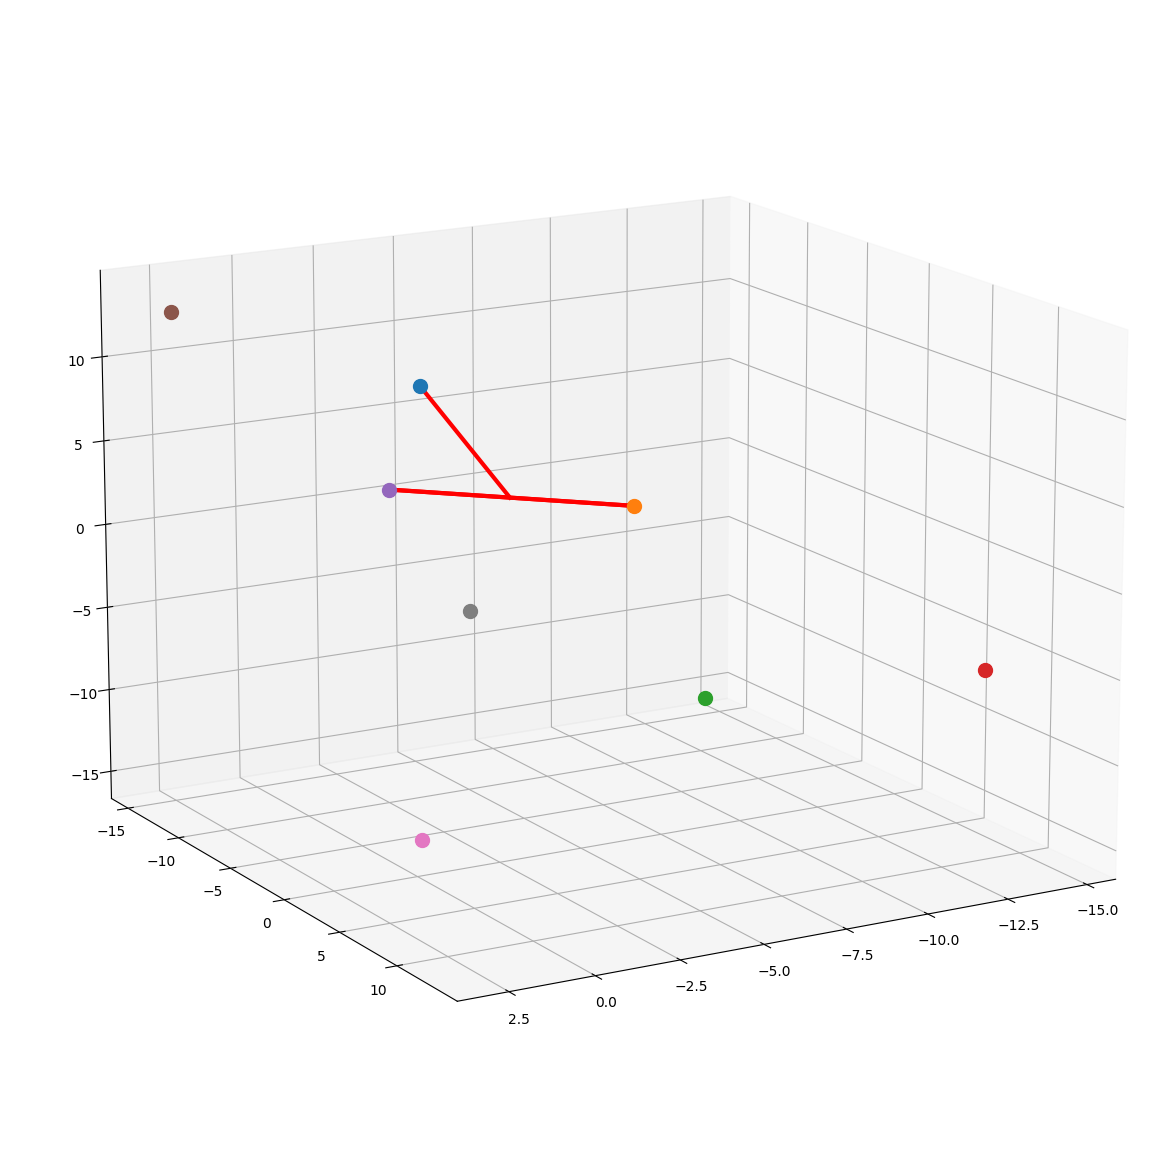
\includegraphics[width=\linewidth]{kd_tree_progress_img0_branches.png}
            \caption{Depth 0}
            \end{subfigure}%
        \hfill
        \begin{subfigure}{.4\textwidth}
            \centering
            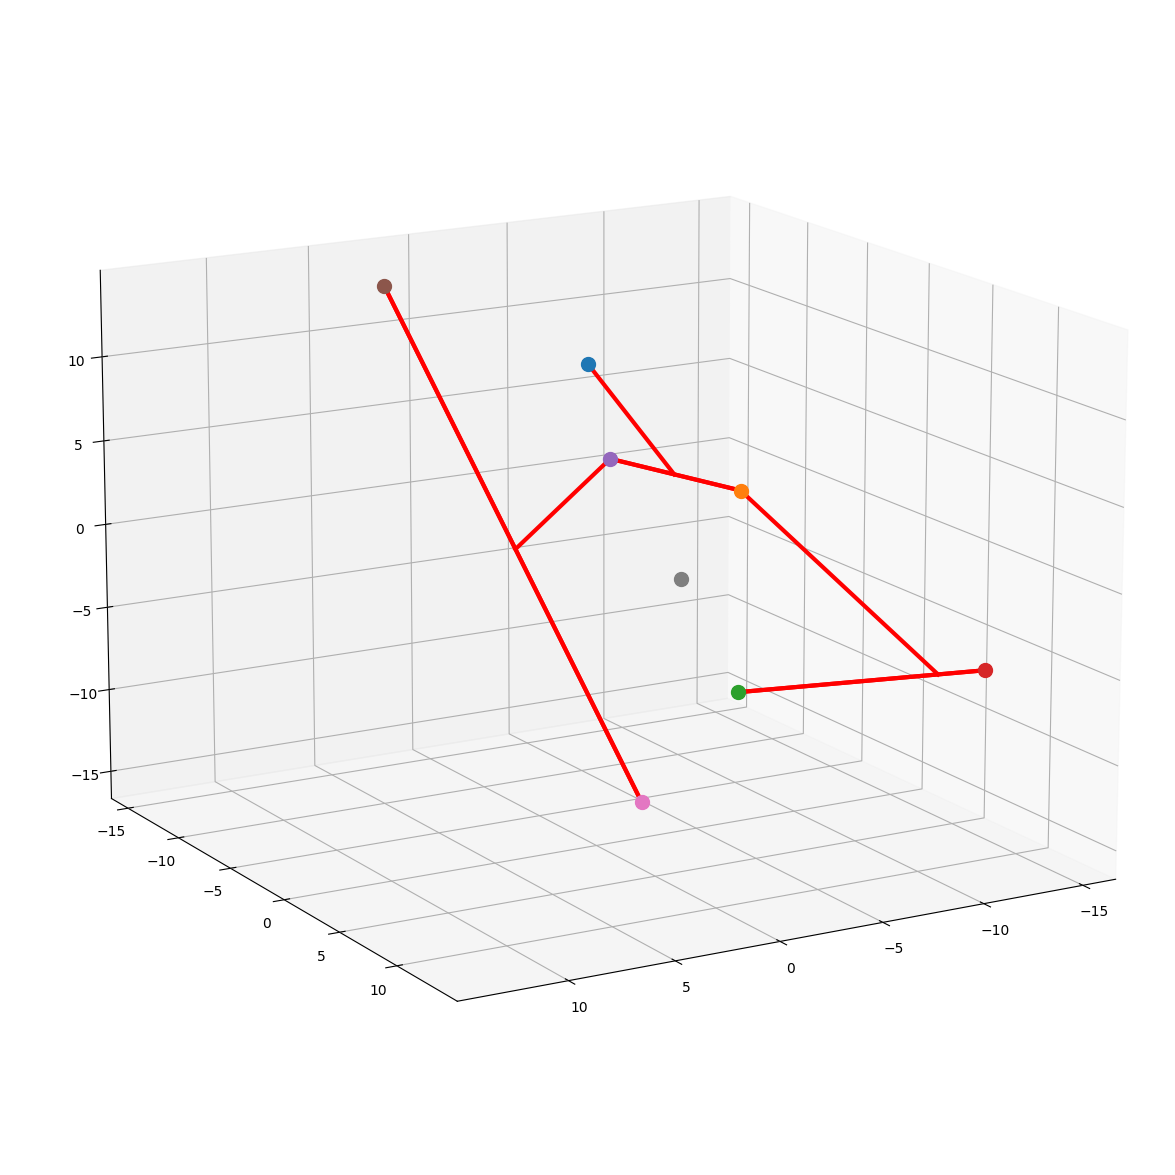
\includegraphics[width=\linewidth]{kd_tree_progress_img1_branches.png}
            \caption{Depth 1}
            \end{subfigure}
        \hfill
        \begin{subfigure}{.4\textwidth}
            \centering
            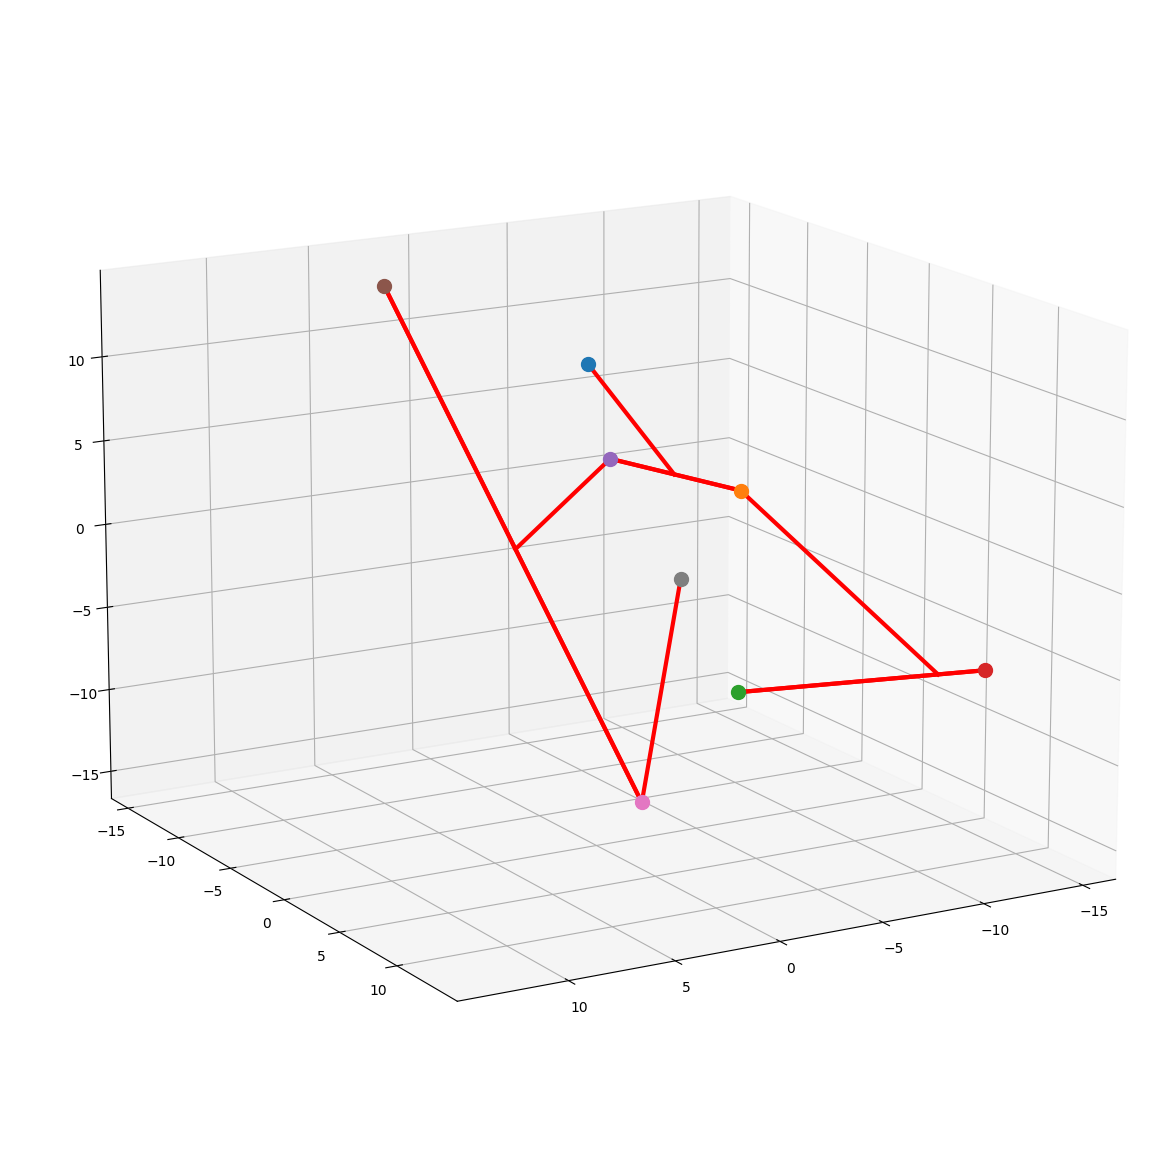
\includegraphics[width=\linewidth]{kd_tree_progress_img2_branches.png}
            \caption{Depth 2}
        \end{subfigure}
    }
    \caption{The same \kdtree{} shown in Figure \ref{fig:kdtree_surfaces_progression} (branches representation).}
    \label{fig:kdtree_branches_progression}
\end{figure}

\section{Parallel algorithm and implementation} \label{sec:algorithm}
First of all we briefly describe the parallel algorithm; then we talk a little
bit about some technicalities needed to glue everything in the two frameworks
taken into account; finally we procede with some words and motivations regarding
how we represented the dataset in our code and which data structures we used.

\subsection{Algorithm}
The following algorithm is a very simple codification of the definition proposed in
Section \ref{sec:intro}:
\begin{algorithm}
    \SetAlgoLined
    \caption{Parallel \kdtree{} growth}\label{alg:parallel_algorithm}
    \KwData{$P = \{p_1, \dots, p_n\}, \ell$}
    $i \gets i(\ell)$ like in (\ref{eq:axis_criteria})\; \label{alg:first}
    Find the median point $p_m$ against the axis $i$\;
    Assign the right branch (i.e. $P_2$) to another parallel worker (if available)\;
    $P \gets P_1, \ell \gets \ell + 1$\;
    Go back to Line \ref{alg:first}\;
\end{algorithm}

The exact definition of ``parallel worker'' depends on the parallel framework
used to compile and run the code:
\begin{itemize}
    \item MPI $\to$ a parallel worker is one of the MPI processes employed to run the code;
    \item OpenMP $\to$ a parallel worker is an OMP thread.
\end{itemize}

It's worth noting that these kind of resources are not unlimited: in case no
parallel workers are available we procede in a serial way, with two recursive
calls to the function which we use to generate the \kdtree{} for both the left
and right branch. This kind of setting requires a more refined approach if
MPI is used (OpenMP is quite convenient in this case), and we will now spend
some words on this.

\subsection{The problem of the ``next'' rank} \label{sec:next_rank}
Whenever we want to communicate something from an MPI process to another, we
need to know precisely what we want to send and what's the process
(i.e. the rank) we want to communicate with. Since in principle we are going to
have multiple processes which want to communicate with multiple children
processes, we needed some way to determine without conflicts the rank of an
idle process, namely a process which is able to take on a branch of the two
branches generated by the current process. Two ideas emerged, which we present
briefly. The first one is a \emph{master-slave}  approach, i.e. to dedicate a
process to the sole work of load-balancing the computation between all the
available parallel workers. A process willing to delegate its right branch to
another MPI process would have needed to:
\begin{enumerate}
    \item Establish a communication with the \emph{master};
    \item Receive the rank of a free MPI process;
    \item Establish a communication with the chosen MPI process;
    \item Send $P_2$.
\end{enumerate}

We had the feeling that this kind of setting would have incremented by 2 units
the number of communications needed to delegate a branch to another process, and
would have made an MPI process totally unusable to the actual purpose of growing
the \kdtree{}; however, the code would have been most likely very elegant and
understandable. Nonetheless we decided to pursue another approach: an
``hardcoded'' protocol. A parent process knows right off the bat the rank
of a child process which is idle and willing to process a branch, and only that
parent process (due to the protocol) is able to communicate with that process.
The rank is computed via some very simple arithmetic operations. The code
becomes less readable, but no-one is going to notice since we decided to hide
this kind of complexity behind a function.

We briefly describe the protocol we employed in our code with a practical
example, let's say sat we have 11 MPI processes (0 being the main process),
which we represent as follows:

\begin{figure}[H]
    \centering
    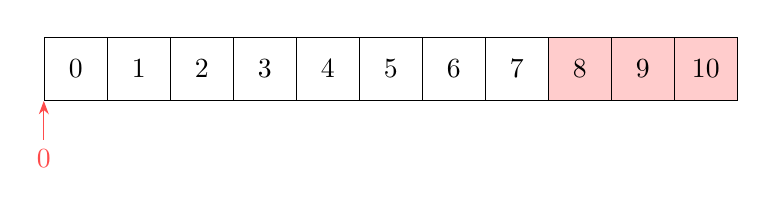
\begin{tikzpicture}
        \matrix (A) [matrix of nodes, nodes={draw, minimum size=8mm},
            column sep=-\pgflinewidth]{
            0 & 1 & 2 & 3 & 4 & 5 & 6 & 7 & |[draw,fill=red!20]|8 & |[draw,fill=red!20]|9 & |[draw,fill=red!20]|10\\};
        \foreach \i [evaluate=\i as \ni using {int(\i)}, evaluate=\i as \ntext using {int(\i-1)}] in {1}
            \draw [{Stealth}-, red!70] (A-1-\ni.south west)--++(-90:5mm) node[below] {0};
    \end{tikzpicture}
\end{figure}

The red arrow pointing to \fbox{0} means that at this point only \fbox{0} is
running, while the other MPI processes are idle, waiting for some branch to be
assigned to them. The number below the arrow refers to the current depth of the
three processed by the process that the arrow is pointing to. Also, at this
point the whole dataset is assigned to \fbox{0}. This is equivalent to
``Depth 0'' in Figure \ref{fig:kdtree_surfaces_progression} and
\ref{fig:kdtree_branches_progression}. Note that \fbox{8}, \fbox{9}, \fbox{10}
are highlighted in red. We call them \texttt{surplus\_workers} for reasons which
will be clarified in some lines.

At this point \fbox{0} executes Algorithm \ref{alg:parallel_algorithm},
which means that the left branch generated (i.e. $P_1$) is recursively assigned
to \fbox{0}. How do we choose the process that receives the right branch (i.e.
$P_2$)? We consider the set of available processes (i.e. those which are not
highlighted), we split it in two equal halves and we assign $P_2$ to the first
process of the right branch (i.e. \fbox{4}):

\begin{figure}[H]
    \centering
    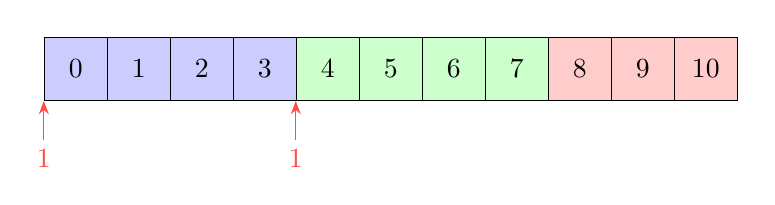
\begin{tikzpicture}
        \matrix (A) [matrix of nodes, nodes={draw, minimum size=8mm},
            column sep=-\pgflinewidth]{
                |[draw,fill=blue!20]|0 & |[draw,fill=blue!20]|1 & |[draw,fill=blue!20]|2 & |[draw,fill=blue!20]|3 & |[draw,fill=green!20]|4 & |[draw,fill=green!20]|5 & |[draw,fill=green!20]|6 & |[draw,fill=green!20]|7 & |[draw,fill=red!20]|8 & |[draw,fill=red!20]|9 & |[draw,fill=red!20]|10\\};
        \foreach \i [evaluate=\i as \ni using {int(\i)},
                        evaluate=\i as \ntext using {int(\i-1)}] in {1,5}
            \draw [{Stealth}-, red!70] (A-1-\ni.south west)--++(-90:5mm) node[below] {1};
    \end{tikzpicture}
\end{figure}

Now we have two processes working in parallel, processing two different parts of
the dataset. We keep splitting the work in the exact same way:

\begin{figure}[H]
    \centering
    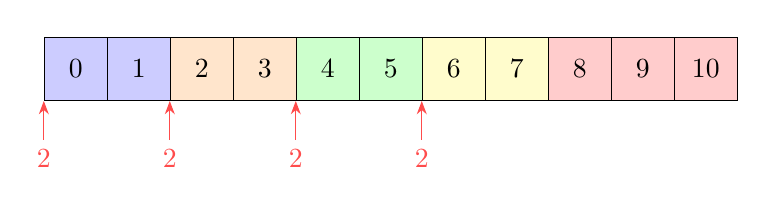
\begin{tikzpicture}
        \matrix (A) [matrix of nodes, nodes={draw, minimum size=8mm},
            column sep=-\pgflinewidth]{
                |[draw,fill=blue!20]|0 & |[draw,fill=blue!20]|1 & |[draw,fill=orange!20]|2 & |[draw,fill=orange!20]|3 & |[draw,fill=green!20]|4 & |[draw,fill=green!20]|5 & |[draw,fill=yellow!20]|6 & |[draw,fill=yellow!20]|7 & |[draw,fill=red!20]|8 & |[draw,fill=red!20]|9 & |[draw,fill=red!20]|10\\};
        \foreach \i [evaluate=\i as \ni using {int(\i)},
                        evaluate=\i as \ntext using {int(\i-1)}] in {1,3,5,7}
            \draw [{Stealth}-, red!70] (A-1-\ni.south west)--++(-90:5mm) node[below] {2};
    \end{tikzpicture}
\end{figure}

At this point we have four processes working in parallel (\fbox{0}, \fbox{2},
\fbox{4}, \fbox{6}) on the second level of the tree. Fast forward, we reach the
following situation:

\begin{figure}[H]
    \centering
    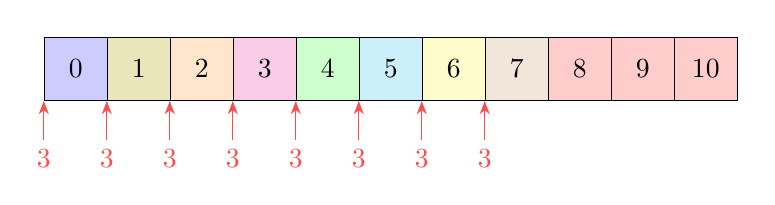
\begin{tikzpicture}
        \matrix (A) [matrix of nodes, nodes={draw, minimum size=8mm},
            column sep=-\pgflinewidth]{
                |[draw,fill=blue!20]|0 & |[draw,fill=olive!20]|1 & |[draw,fill=orange!20]|2 & |[draw,fill=magenta!20]|3 & |[draw,fill=green!20]|4 & |[draw,fill=cyan!20]|5 & |[draw,fill=yellow!20]|6 & |[draw,fill=brown!20]|7 & |[draw,fill=red!20]|8 & |[draw,fill=red!20]|9 & |[draw,fill=red!20]|10\\};
        \foreach \i [evaluate=\i as \ni using {int(\i)},
                        evaluate=\i as \ntext using {int(\i-1)}] in {1,2,3,4,5,6,7,8}
            \draw [{Stealth}-, red!70] (A-1-\ni.south west)--++(-90:5mm) node[below] {3};
    \end{tikzpicture}
\end{figure}

We now have three idle proccesses (\fbox{8}, \fbox{9}, \fbox{10}), which are
clearly not enough to parallelize entirely a new level. Even though the
performance gain we get by using also these \texttt{surplus\_workers} is not
so influential (we have to wait the slowest parts of the tree to be completed)
we decided to assign them left-to-right to the other processes. In this case
only \fbox{0}, \fbox{1} and \fbox{2} would get a \texttt{surplus\_workers}
(respectively \fbox{8}, \fbox{9} and \fbox{10}). Therefore the final situation
is:

\begin{figure}[H]
    \centering
    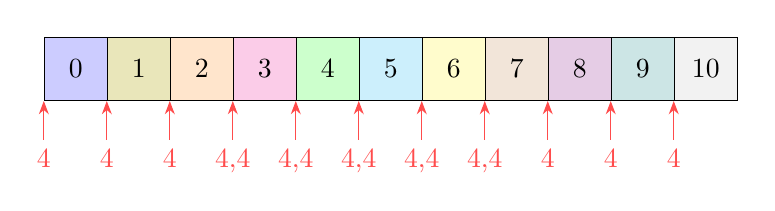
\begin{tikzpicture}
        \matrix (A) [matrix of nodes, nodes={draw, minimum size=8mm},
            column sep=-\pgflinewidth]{
                |[draw,fill=blue!20]|0 & |[draw,fill=olive!20]|1 & |[draw,fill=orange!20]|2 & |[draw,fill=magenta!20]|3 & |[draw,fill=green!20]|4 & |[draw,fill=cyan!20]|5 & |[draw,fill=yellow!20]|6 & |[draw,fill=brown!20]|7 & |[draw,fill=violet!20]|8 & |[draw,fill=teal!20]|9 & |[draw,fill=lightgray!20]|10\\};
        \foreach \i [evaluate=\i as \ni using {int(\i)},
                        evaluate=\i as \ntext using {int(\i-1)}] in {1,2,3,9,10,11}
            \draw [{Stealth}-, red!70] (A-1-\ni.south west)--++(-90:5mm) node[below] {4};
        \foreach \i [evaluate=\i as \ni using {int(\i)},
            evaluate=\i as \ntext using {int(\i-1)}] in {4,5,6,7,8}
            \draw [{Stealth}-, red!70] (A-1-\ni.south west)--++(-90:5mm) node[below] {4,4};
    \end{tikzpicture}
\end{figure}

As you can see \fbox{3}, \fbox{4}, \fbox{5}, \fbox{6}, \fbox{7} receive both the
branches they spawned, while the other processes receive only one. From now on
we do not have other MPI processes, therefore the computation proceeds serially.

As we mentioned earlier OpenMP does not requires these technicalities since we
employed OpenMP \emph{Tasks} to parallelize the computation. Each time we need
to assign a branch to another thread we just spawn a new task, and then process
the remaining branch on this thread. We employed the modifier \texttt{final}
to disable spawning new tasks when we know that no more threads are available
since otherwise the newly spawned task would have to wait until a new thread
became available; also spawning OpenMP tasks without control usually leads to
worse performance due the incremented orchestration overhead
\cite{hager2010introduction}. Checking whether new threads are available is done
almost in the same way we presented above (even though we do not need to compute
the rank of the next threads). The same mechanism of \texttt{surplus\_workers}
is employed to overcome the issues which emerges when the number of parallel
workers is not exactly a power of 2.

\subsection{Merging}
Another difficulty in the usage of MPI is the fact that each process that
delegated one or more branches to other MPI processes needs to recover and
reconstruct a \kdtree{} starting from the portion of tree produced by child
processes. This operation is analogous to the \texttt{merge} subroutine which is
used in common implementations of \emph{Merge-Sort}
\cite{cormen2009introduction}. Indeed in our code the function which
encapsulates this operation is called \texttt{merge\_kd\_trees}. Note that
\emph{merging} is not required if we use OpenMP, unless we employ some
particular strategy for writing into the 1D array which represents the
\kdtree{} in memory (for instance, see Section \ref{sec:false_sharing}).

Summing up, the abstract algorithm for the growth of \kdtree{} (for which we
presented a very general pseudocode in Algorithm \ref{alg:parallel_algorithm})
must be extended as follows if MPI is used:

\begin{algorithm}[H]
    \SetAlgoLined
    \KwData{$P = \{p_1, \dots, p_n\}, \ell$, \texttt{m\_rank}}
    \caption{Parallel \kdtree{} growth (MPI)}\label{alg:parallel_algorithm_mpi}
    Run Algorithm \ref*{alg:parallel_algorithm}\;
    \texttt{KDT} $\gets$ \kdtree{} rooted in the first fully serial level computed by \texttt{m\_rank}\;
    \ForEach{$r \in \mathcal{C}_{\texttt{m\_rank}}^{-1}$}
        {
            \texttt{right\_kdt} $\gets$ \kdtree{} generated by process $r$\;
            \texttt{KDT} $\gets$ \texttt{merge\_kd\_trees}(\texttt{KDT}, \texttt{right\_kdt})\;
        }
\end{algorithm}

As you can see we procede in a bottom-up fashion and locate the first fully
serial level computed by this process (i.e. the first level of the \kdtree{}
such that no branches have been delegated to another process). Then we procede
towards the root of the \kdtree{} querying the processes which received some
branch from \texttt{m\_rank} for the result of their computation. We refer as
$\mathcal{C}_{\texttt{m\_rank}}$ to the list of child processes of
\texttt{m\_rank}, and $\mathcal{C}_{\texttt{m\_rank}}^{-1}$ means that we
traverse that list in reverse order (i.e. the last inserted child is the first
to be queried).

\subsection{Fixing \emph{false-sharing}} \label{sec:false_sharing}
Not only MPI determines more techical challenges than expected: OpenMP does too.
Until now we managed to stay very high level ignoring technical details
like, for instance, how the \kdtree{} is stored in the memory of a process. We
now state that the in-memory representation is a 1D array of
\texttt{std::optional<DataPoint>}. \texttt{DataPoint} is a class which contains
a pointer to a 1D array of \texttt{float} or \texttt{double} values (depending
on a compilation flag). This pointer points to the appropriate position inside a
big 1D array of values which contains all the components of all the datapoints
(note that this means that each \texttt{DataPoint} does not ``own'' its data, so
it's not responsible of deleting). We depict this setting in an image to
clarify:
\begin{figure}[H]
    \centering
    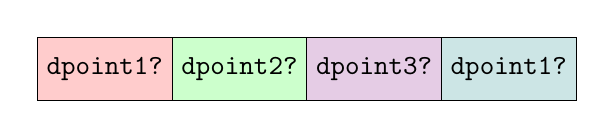
\begin{tikzpicture}
        \matrix (A) [matrix of nodes, nodes={draw, minimum size=8mm},
            column sep=-\pgflinewidth]{
                |[draw,fill=red!20]|\texttt{dpoint1?} & |[draw,fill=green!20]|\texttt{dpoint2?} & |[draw,fill=violet!20]|\texttt{dpoint3?} & |[draw,fill=teal!20]|\texttt{dpoint1?}\\};
    \end{tikzpicture}
\end{figure}
\begin{figure}[H]
    \centering
    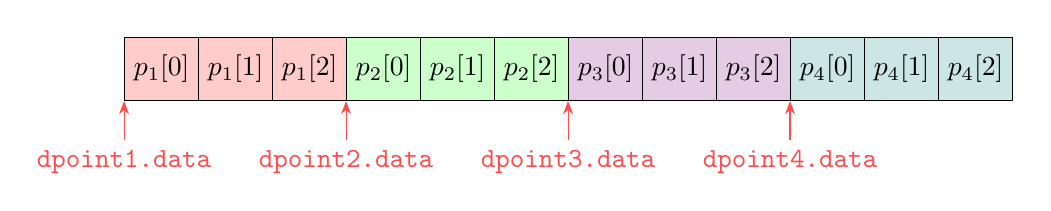
\begin{tikzpicture}
        \matrix (A) [matrix of nodes, nodes={draw, minimum size=8mm},
            column sep=-\pgflinewidth]{
                |[draw,fill=red!20]|$p_1[0]$ & |[draw,fill=red!20]|$p_1[1]$ & |[draw,fill=red!20]|$p_1[2]$ & |[draw,fill=green!20]|$p_2[0]$ & |[draw,fill=green!20]|$p_2[1]$ & |[draw,fill=green!20]|$p_2[2]$ & |[draw,fill=violet!20]|$p_3[0]$ & |[draw,fill=violet!20]|$p_3[1]$ & |[draw,fill=violet!20]|$p_3[2]$ & |[draw,fill=teal!20]|$p_4[0]$ & |[draw,fill=teal!20]|$p_4[1]$ & |[draw,fill=teal!20]|$p_4[2]$\\};
        \draw [{Stealth}-, red!70] (A-1-1.south west)--++(-90:5mm) node[below] {\texttt{dpoint1.data}};
        \draw [{Stealth}-, red!70] (A-1-4.south west)--++(-90:5mm) node[below] {\texttt{dpoint2.data}};
        \draw [{Stealth}-, red!70] (A-1-7.south west)--++(-90:5mm) node[below] {\texttt{dpoint3.data}};
        \draw [{Stealth}-, red!70] (A-1-10.south west)--++(-90:5mm) node[below] {\texttt{dpoint4.data}};
    \end{tikzpicture}
\end{figure}

Moreover the class \texttt{DataPoint} defines come convenient methods which are
used to simplify the code. We decided to use \texttt{std::optional} since in
principle some values of the tree might be empty: this happens because we
enforce the rule that all the nodes of the \kdtree{} (except the leaves) must
have exactly two children. We made this decision in order to simplify the
communication protocol between different MPI processes/OMP threads. However
these details might be ignored since they do not determine any particular
performance improvement, and are mere design choices. For this reason from now
on we're going to consider the ``local'' \kdtree{} (i.e. that grown by a single
parallel worker) as a 1D simple array of ``points''.

Inside this 1D array, $2^\ell$ consecutive points represent a level of the
tree, where $\ell$ is the depth (i.e. distance from the root) of the level.
It has been experimentally observed (via the operator \texttt{sizeof}) that when
the data type is \texttt{float} and each data point has three components, each
item in the 1D array has size 16 bytes. We visualize this setting in the
following image (each $p_i$ in this case is an ``empty spot'' to be filled with
a data point from the dataset):

\begin{figure}[H]
    \centering
    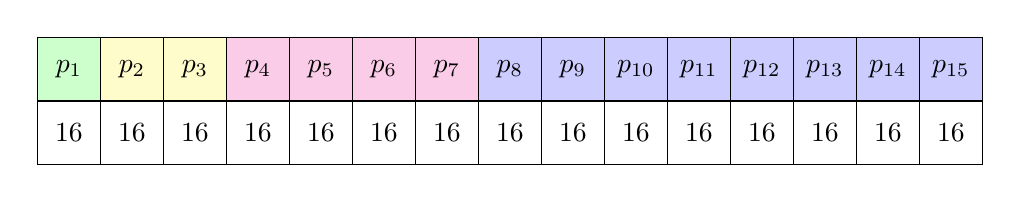
\begin{tikzpicture}
        \matrix (A) [matrix of nodes, nodes={draw, minimum size=8mm},
            column sep=-\pgflinewidth]{
                |[draw,fill=green!20]|$p_1$ & |[draw,fill=yellow!20]|$p_2$ & |[draw,fill=yellow!20]|$p_3$ & |[draw,fill=magenta!20]|$p_4$ & |[draw,fill=magenta!20]|$p_5$ & |[draw,fill=magenta!20]|$p_6$ & |[draw,fill=magenta!20]|$p_7$ & |[draw,fill=blue!20]|$p_8$ & |[draw,fill=blue!20]|$p_9$ & |[draw,fill=blue!20]|$p_{10}$ & |[draw,fill=blue!20]|$p_{11}$ & |[draw,fill=blue!20]|$p_{12}$ & |[draw,fill=blue!20]|$p_{13}$ & |[draw,fill=blue!20]|$p_{14}$ & |[draw,fill=blue!20]|$p_{15}$\\
                16 & 16 & 16 & 16 & 16 & 16 & 16 & 16 & 16 & 16 & 16 & 16 & 16 & 16 & 16\\};
    \end{tikzpicture}
\end{figure}

We now observe that the \emph{naive} write mode is very inconvenient for OpenMP,
if the 1D array which represents the \kdtree{} is shared among all the parallel
OMP threads. ``\emph{naive} write mode'' means that each thread writes all the
points in their proper location inside the 1D array. This means that we could
virtually observe all the OMP threads writing in the same \kdtree{} level at
the same time, but in different cells of the array. However if we consider
a cache line to be 128 bytes long, this means that we could have 8 OMP threads
writing concurrently to that same memory address window, which results in very
poor performance when we take into account cache coherency
\cite{hager2010introduction}. Note that this is definitely not a problem if we
use MPI, since memory is distributed rather than shared.

In order to fix \emph{false-sharing} we introduced a compilation flag
(\texttt{ALTERNATIVE\_SERIAL\_WRITE}) which allows to select a different write
mode which minimzes the number of concurrent writes on addresses which might
belong to the same cache line. We briefly describe this method using some
images. Let's consider again the 1D array depicted above.

\begin{figure}[H]
    \centering
    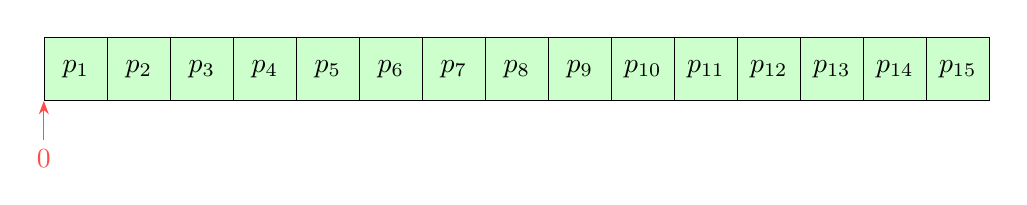
\begin{tikzpicture}
        \matrix (A) [matrix of nodes, nodes={draw, minimum size=8mm},
            column sep=-\pgflinewidth]{
                |[draw,fill=green!20]|$p_1$ & |[draw,fill=green!20]|$p_2$ & |[draw,fill=green!20]|$p_3$ & |[draw,fill=green!20]|$p_4$ & |[draw,fill=green!20]|$p_5$ & |[draw,fill=green!20]|$p_6$ & |[draw,fill=green!20]|$p_7$ & |[draw,fill=green!20]|$p_8$ & |[draw,fill=green!20]|$p_9$ & |[draw,fill=green!20]|$p_{10}$ & |[draw,fill=green!20]|$p_{11}$ & |[draw,fill=green!20]|$p_{12}$ & |[draw,fill=green!20]|$p_{13}$ & |[draw,fill=green!20]|$p_{14}$ & |[draw,fill=green!20]|$p_{15}$\\};
            \foreach \i [evaluate=\i as \ni using {int(\i)},
                evaluate=\i as \ntext using {int(\i-1)}] in {1}
                \draw [{Stealth}-, red!70] (A-1-\ni.south west)--++(-90:5mm) node[below] {0};
    \end{tikzpicture}
\end{figure}

The OMP thread \texttt{thread0} is assigned the dataset $P$ and has the duty to
fill the big green array above in such a way that it's easy to recover the
\kdtree{} corresponding to $P$ afterwards. Therefore it dermines the median
point and splits $P$ into $P_1$ and $P_2$. It also places the median point into
$p_1$. In order to reduce the number of concurrent write on the same cache line,
we divide the remaining array in two halves, and we make sure that only
\texttt{thread0} (and its descendants) can write in the left part, and only
\texttt{thread1} (and its descendants) can write on the right part (we assume
that \texttt{thread1} takes on the task associated with right branch $P_2$).
The situation now looks like this:
\begin{figure}[H]
    \centering
    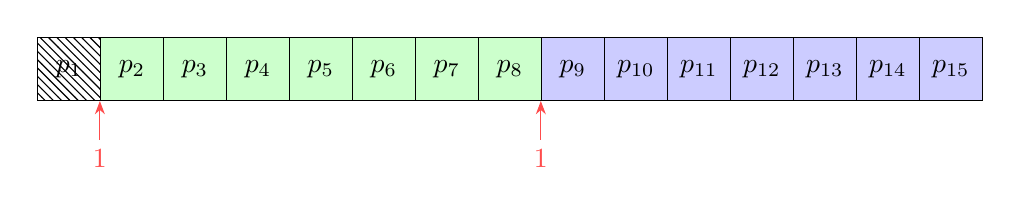
\begin{tikzpicture}
        \matrix (A) [matrix of nodes, nodes={draw, minimum size=8mm},
            column sep=-\pgflinewidth]{
                |[draw,pattern=north west lines]|$p_1$ & |[draw,fill=green!20]|$p_2$ & |[draw,fill=green!20]|$p_3$ & |[draw,fill=green!20]|$p_4$ & |[draw,fill=green!20]|$p_5$ & |[draw,fill=green!20]|$p_6$ & |[draw,fill=green!20]|$p_7$ & |[draw,fill=green!20]|$p_8$ & |[draw,fill=blue!20]|$p_9$ & |[draw,fill=blue!20]|$p_{10}$ & |[draw,fill=blue!20]|$p_{11}$ & |[draw,fill=blue!20]|$p_{12}$ & |[draw,fill=blue!20]|$p_{13}$ & |[draw,fill=blue!20]|$p_{14}$ & |[draw,fill=blue!20]|$p_{15}$\\};
            \foreach \i [evaluate=\i as \ni using {int(\i)},
                evaluate=\i as \ntext using {int(\i-1)}] in {2,9}
                \draw [{Stealth}-, red!70] (A-1-\ni.south west)--++(-90:5mm) node[below] {1};
    \end{tikzpicture}
\end{figure}

We keep writing the median point on the first memory address in the subset
assigned to the thread, and splitting the remaining memory between the two
threads that process the left and right branches generated:
\begin{figure}[H]
    \centering
    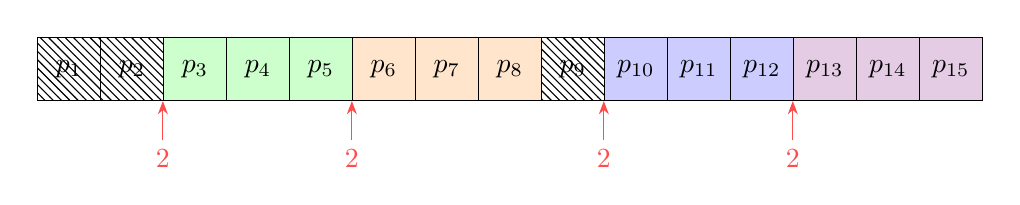
\begin{tikzpicture}
        \matrix (A) [matrix of nodes, nodes={draw, minimum size=8mm},
            column sep=-\pgflinewidth]{
                |[draw,pattern=north west lines]|$p_1$ & |[draw,pattern=north west lines]|$p_2$ & |[draw,fill=green!20]|$p_3$ & |[draw,fill=green!20]|$p_4$ & |[draw,fill=green!20]|$p_5$ & |[draw,fill=orange!20]|$p_6$ & |[draw,fill=orange!20]|$p_7$ & |[draw,fill=orange!20]|$p_8$ & |[draw,pattern=north west lines]|$p_9$ & |[draw,fill=blue!20]|$p_{10}$ & |[draw,fill=blue!20]|$p_{11}$ & |[draw,fill=blue!20]|$p_{12}$ & |[draw,fill=violet!20]|$p_{13}$ & |[draw,fill=violet!20]|$p_{14}$ & |[draw,fill=violet!20]|$p_{15}$\\};
            \foreach \i [evaluate=\i as \ni using {int(\i)},
                evaluate=\i as \ntext using {int(\i-1)}] in {3,6,10,13}
                \draw [{Stealth}-, red!70] (A-1-\ni.south west)--++(-90:5mm) node[below] {2};
    \end{tikzpicture}
\end{figure}

This is not very meaningful when the number of points in the levels of the tree
are small like in this example, but the situation changes radically as we
increase the height of the \kdtree{}. Clearly we need to re-write the \kdtree{}
in the expected form afterwards: this is something that may reduce, or even
nullify, the performance gains which we get by removing \emph{false-sharing}.

Another possible solution is introducing some \emph{padding}
\cite{hager2010introduction}, i.e. artificially augmenting the number of
components for each data point in order to reduce the number of threads possibly
writing on the same cache line . For instance, if we manage to increase the size
of each item in the array from 16 to 64 bytes rwe would risk writing
concurrently on the same cache line with two threads instead of eight.

\subsection{Improving the memory access pattern} \label{sec:mem_acc_pattern}
The most computationally intensive line in our code is the call to
\texttt{std::nth\_element} which is used to find the median element of a set of
points in a branch. This function is called exactly one time per branch, and its
computational complexity is $O(n)$. But rather than the computational complexity
we look at the memory access pattern: a bad access pattern is capable to ruin
performances potentially worse than an excessive complexity
\cite{hager2010introduction}. This is particularly true since the body of the
function \texttt{std::nth\_element} involves multiple comparisons between the
data points in the branch against the chosen axis $i$. Since we're only
interested in the $i$-th component for those comparisons, storing and accessing
the data points in this way:
\begin{figure}[H]
    \centering
    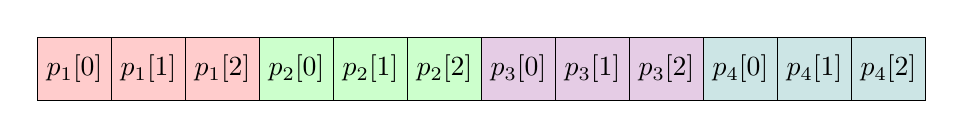
\begin{tikzpicture}
        \matrix (A) [matrix of nodes, nodes={draw, minimum size=8mm},
            column sep=-\pgflinewidth]{
                |[draw,fill=red!20]|$p_1[0]$ & |[draw,fill=red!20]|$p_1[1]$ & |[draw,fill=red!20]|$p_1[2]$ & |[draw,fill=green!20]|$p_2[0]$ & |[draw,fill=green!20]|$p_2[1]$ & |[draw,fill=green!20]|$p_2[2]$ & |[draw,fill=violet!20]|$p_3[0]$ & |[draw,fill=violet!20]|$p_3[1]$ & |[draw,fill=violet!20]|$p_3[2]$ & |[draw,fill=teal!20]|$p_4[0]$ & |[draw,fill=teal!20]|$p_4[1]$ & |[draw,fill=teal!20]|$p_4[2]$\\};
    \end{tikzpicture}
\end{figure}
is probably suboptimal, since every time we access $p_k[i]$ we load in the cache
a nearboroughood of $p_k[i]$, i.e. $p_k[i-1], p_k[i+1], \dots$.
For this reason we decided to try a different arrangement in memory. A new
copy of the array of data points was needed since we receive the data from the
``user'' in a 1D array which looks like the one in the image above. We depict
the new arrangement:
\begin{figure}[H]
    \centering
    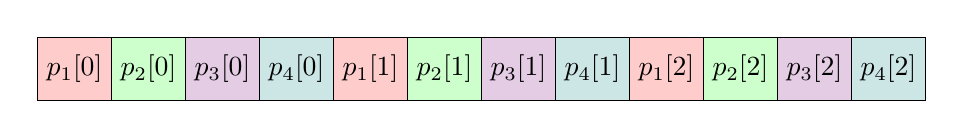
\begin{tikzpicture}
        \matrix (A) [matrix of nodes, nodes={draw, minimum size=8mm},
            column sep=-\pgflinewidth]{
                |[draw,fill=red!20]|$p_1[0]$ & |[draw,fill=green!20]|$p_2[0]$ & |[draw,fill=violet!20]|$p_3[0]$ & |[draw,fill=teal!20]|$p_4[0]$ & |[draw,fill=red!20]|$p_1[1]$ & |[draw,fill=green!20]|$p_2[1]$ & |[draw,fill=violet!20]|$p_3[1]$ & |[draw,fill=teal!20]|$p_4[1]$ & |[draw,fill=red!20]|$p_1[2]$ & |[draw,fill=green!20]|$p_2[2]$ & |[draw,fill=violet!20]|$p_3[2]$ & |[draw,fill=teal!20]|$p_4[2]$\\};
    \end{tikzpicture}
\end{figure}
Now a call to \texttt{std::nth\_element} would most likely have a much smaller
number of \emph{cache misses}, since the ``interesting'' addresses in the array
below (for a given axis $i$) are close to each other in memory.

This approach did not pay unfortunately, since a single experiment with 8 MPI
processes and a dataset of 100'000'000 data points each having 3 components
took about 163\% the time needed to grow the tree before the modification on the
same dataset. For this reason we decided to pause this improvement, a profiler
could probably tell us what's happening inside the code.

\section{Performance model and results} \label{sec:performance}
On the basis of the discussion we developed in Section \ref{sec:algorithm} we
propose the following performance model, which we are going to compare against
the experimental results we obtained in several runs of our code:
\begin{align}\label{eq:perf_model}
    T(P,N) = &t(\phi(P,N)) + pc(P,N) + cp(P,N)\notag\\
    &+ \texttt{parallel\_split}(P,N) + w(P,N) + \texttt{merge}(P, N)
\end{align}
This equation tries to model the time needed for a worker to grow a \kdtree{}.
For simplicity we assume that $N = 2^k, k \in \mathbb{N}$, but it's not
difficult to generalize the model with a few more technicalities. We briefly
explain the meaning of the symbols in (\ref*{eq:perf_model}):
\begin{itemize}
    \item T(P,N) is the time needed to grow a \kdtree{} having $N$ elements
    on $P$ parallel workers;
    \item t(N) is the time needed to grow serially a \kdtree{} having $N$
    elements;
    \item $\phi(P,N)$ is the number of elements in the first non-parallelizable
    branch generated by a worker which in principle can parallelize the
    generation of a \kdtree{} having $N$ elements using $P$ workers;
    \item $pc(P,N)$ is the time needed to communicate one branch per level to
    another worker, until the first non-parallelizable level is reached;
    \item $cp(P,N)$ is the time needed to retrieve the grown \kdtree{} from the
    workers which received a branch from this worker;
    \item $w(P,N)$ is the time that this worker needs to wait before the
    children branches complete their work;
    \item $\texttt{merge(P,N)}$ is the time needed to build the \kdtree{}
    starting from the serial branch grown by this worker and the branches
    delegated to other workers;
    \item $\texttt{parallel\_split}(P,N)$ is the time needed to split the data
    in branches (one of them is delegated to another worker) before the first
    non-parallelizable level.
\end{itemize}

Note that $pc \equiv 0, cp \equiv 0$ if we use OpenMP, but this is probably a
coarse approximation since there are hidden costs involved, for instance in
maintaining cache coherency (we spent some words on this problem in Section
\ref{sec:false_sharing}). We simplify the model and assume the same cost of
communication for sending a branch and receiving the corresponding grown
\kdtree{}, which we call \texttt{comm}$(P,N)$.

The following relation holds:
\begin{gather*}
    w(P,N) = \begin{cases}
        0 &\text{ if } P = 2^k, k \in \mathbb{N}\\
        t(\phi(P,N)) &\text{otherwise}
    \end{cases}
\end{gather*}
The first condition means that we can parallelize in the exact same way
all the regions of the \kdtree{}, while the latter means that some parts cannot
be parallelized and therefore need to start the serial growth of the tree one
level before the others (see \texttt{surplus\_workers} in Section
\ref{sec:next_rank}). Therefore we write $w(P,N) = \alpha(P)\phi(P,N)$ where
$\alpha(P)$ is 0 if $P$ is a power of 2, and 1 otherwise.

Recalling the serial algorithm which we employ to compute the \kdtree{}, the
complexity is the same of \emph{Merge-Sort} (this can be shown via the
\emph{Master theorem}), namely $t(N) \in O(N \log N)$. Therefore we assume that
$t(N) = \beta N \log N$, where $\beta$ is some proportionality constant.

We now look at \texttt{parallel\_split}$(P,N)$ and \texttt{merge}$(P,N)$. The
former consists in the iterated application of \texttt{std::nth\_element} to
datasets whose size is $N, N/2, N/4, ..., N2^{-\log_2(\hat{P})}$, where
$\hat{P}$ is the greatest power of 2 lower than or equal to $P$. Since the
complexity of \texttt{std::nth\_element} is $O(N)$, using the value of the
summation of a geometric sum and introducing a proportionality constant
$\gamma_1$, we obtain:
\begin{align} \label{eq:parallel_split_relation}
    \texttt{parallel\_split}(P,N) &= \gamma_1 \sum_{i=0}^{\log_2(\hat{P})} \frac{N}{2^i}\\
    &= \gamma_1 N \sum_{i=0}^{\log_2(\hat{P})} \frac{1}{2^i}\\
    &= \gamma_1 N (2 - 2^{-\log_2(\hat{P})})\\
    &= \gamma_1 N \left(2 - \frac{1}{\hat{P}}\right)
\end{align}
Since \texttt{merge}$(P,N)$ (if we use MPI) consists in a linear scan of the two
branches which comprise a level, iterated for all the levels from the last
parallelizable level to the root, we obtain relation very similar to
(\ref*{eq:parallel_split_relation}):
\begin{gather*}
    \texttt{merge}(P,N) = \gamma_2 N \left(2 - \frac{1}{\hat{P}}\right)
\end{gather*}
If we use OpenMP no merging is needed (unless we employ the approach
presented in Section \ref{sec:false_sharing}), therefore
\texttt{merge}$(P,N) \equiv 0$.

Lastly, we observe that $\phi(P,N) = \frac{N}{\hat{P}}$. At this point we can
express a simplified model based on the assumptions we stated above:
\begin{gather*}
    T(P,N) = \begin{cases}
        (1+\alpha(P)) \beta \frac{N}{\hat{P}} \log \frac{N}{\hat{P}} + 2\texttt{comm}(P,N) + (\gamma_1 + \gamma_2) N \left(2 - \frac{1}{\hat{P}}\right) &\text{(MPI)}\\
        (1+\alpha(P)) \beta \frac{N}{\hat{P}} \log \frac{N}{\hat{P}} + \gamma_1 N \left(2 - \frac{1}{\hat{P}}\right) + \texttt{hidden}(P,N) &\text{(OpenMP)}
    \end{cases}
\end{gather*}
Note that we added an ``hidden cost'' term in OpenMP to remind that OpenMP isn't
just ``MPI \emph{minus} communication'', and the experimental results are going
to remark strongly this fact.

The model testifies that in our experimental results, as we increase the number
of parallel workers $P$, we should observe a steep improvement of the
performance each time $P$ becomes a power of 2. However, the incidence of this
improvement depends on the cost of communication in the MPI case, while in the
OpenMP case the model is most likely unprecise due to unquantified hidden
costs.

Another aspect which remains unexplained by this model is the decrease of
execution time which we are going to observe in the following sections when
we increase the number of parallel workers to a number which is not a power of
2 (for instance, see Figure \ref{fig:strong_scaling}). This is most likely due
to the fact that parallel workers are not working equally fast. This means
that waiting for the computation of the additional (i.e. non-parallelizable)
level of (for instance) 5 or 6 workers is practically not the same of waiting
for the computation of the additional level of one worker, since in the former
case the probability of having a slower worker is much higher. The slower worker
is a \emph{bottleneck}, therefore increasing the number of workers (even though
we do not reach the next power of 2) reduces the probability of having a
bottleneck which stalls the other processes waiting for its portion of the
dataset.

\subsection{Software and hardware employed for the experiments}
In the following sections we are going to present and discuss some experimental
measurements in order to verify the fidelity of our theoretical model. The
measurements have been carried out using a variable number of cores on a single
\emph{Thin} node on \emph{Orfeo}. The code have been compiled using \emph{gcc}
9.3.0, the MPI distribution taken into account is OpenMPI 4.0.3.

All the datasets have been generated using a small Python utility which we wrote
for the purpose. The utility enables the generation of \texttt{.csv} files
containing a random dataset following a \emph{Normal} distribution, with an
arbitrary number of data points (row) having an arbitrary number of
components (columns). In particular for the experiments we fixed the number of
components to 3, while the number of data points varies according to the
experiment.

\subsection{\emph{Strong} and \emph{weak} scalability}
\begin{figure}[t!]
    \centering
    \begin{subfigure}[b]{0.4\textwidth}
        \centering
        \begin{tikzpicture}[scale=0.75]
            \begin{axis}[
                xtick={1,2,4,8,16,24},
                grid=both,
                ylabel={Seconds},
                xlabel={$P$},
                legend cell align={left},
                title={Time needed to grow the \kdtree{}.},
                y label style={at={(axis description cs:0.05,0.5)}}
            ]
            \addplot table[x index=0, y index=1] {plots_data/big_dataset.txt};
            \addplot table[x index=0, y index=2] {plots_data/big_dataset.txt};

            \legend{MPI, OpenMP}
            \end{axis}
        \end{tikzpicture}
    \end{subfigure}
    \hspace{1cm}
    \begin{subfigure}[b]{0.4\textwidth}
        \centering
        \begin{tikzpicture}[scale=0.75]
            \begin{axis}[
                xtick={1,2,4,8,16,24},
                grid=both,
                ylabel={$T(1) / T(P)$},
                xlabel={$P$},
                legend cell align={left},
                title={Parallel speedup (and scalability).},
                legend style={at={(0.5,0.3)},anchor=west},
                y label style={at={(axis description cs:0.08,0.5)}}
            ]
            \addplot table[x index=0, y index=3] {plots_data/big_dataset.txt};
            \addplot table[x index=0, y index=4] {plots_data/big_dataset.txt};

            \legend{MPI, OpenMP}
            \end{axis}
        \end{tikzpicture}
    \end{subfigure}
\caption{Strong scalability of the growth of a \kdtree{} ($N = $ 100'000'000).}
\label{fig:strong_scaling}
\end{figure}
First of all we briefly discuss the \emph{strong scalability} of our code, namely
the performance gain given by the introduction of additional parallel workers
while the problem size stays constant. As you can see in Figure
\ref{fig:strong_scaling} we observe the behavior we expected after the
inspection of the simplified model (i.e. steep improvement everytime we add
$2^k$ processors). Also, we observe that the hidden cost of OpenMP is definitely
not negligible. The slight instability in the OpenMP line could probably mean
that some OMP threads have been paused and assigned to other tasks. Note that
in this case we can observe the effect we forecasted (and explained)
in the last paragraph of the introduction to Section \ref{sec:performance}, i.e.
the improvement of performance even if the number of parallel workers is not
a power of 2.

\begin{figure}[b!]
    \centering
    \begin{subfigure}[b]{0.4\textwidth}
        \centering
        \begin{tikzpicture}[scale=0.75]
            \begin{axis}[
                xtick={1,2,4,8,16,24},
                grid=both,
                ylabel={Seconds},
                xlabel={$P$},
                legend cell align={left},
                title={Time needed to grow the \kdtree{}.},
                legend style={at={(0.2,0.8)},anchor=west},
                y label style={at={(axis description cs:0.05,0.5)}}
            ]
            \addplot table[x index=0, y index=1] {plots_data/weak_scalability.txt};
            \addplot table[x index=0, y index=2] {plots_data/weak_scalability.txt};

            \legend{MPI, OpenMP}
            \end{axis}
        \end{tikzpicture}
    \end{subfigure}
    \hspace{1cm}
    \begin{subfigure}[b]{0.4\textwidth}
        \centering
        \begin{tikzpicture}[scale=0.75]
            \begin{axis}[
                xtick={1,2,4,8,16,24},
                grid=both,
                ylabel={$P T(1) / T(P)$},
                xlabel={$P$},
                legend cell align={left},
                title={Weak scalability, $\alpha = 1$.},
                legend style={at={(0.5,0.2)},anchor=west},
                y label style={at={(axis description cs:0.05,0.5)}}
            ]
            \addplot table[x index=0, y index=3] {plots_data/weak_scalability.txt};
            \addplot table[x index=0, y index=4] {plots_data/weak_scalability.txt};

            \legend{MPI, OpenMP}
            \end{axis}
        \end{tikzpicture}
    \end{subfigure}
    \caption{Weak scalability of the growth of a \kdtree{} for a linearly varying number of elements.}
    \label{fig:weak_scaling}
\end{figure}
In order to evaluate the \emph{weak scalability} of our implementation, we
generated a set $\mathcal{D} = \{d_1.csv, \dots, d_{24}.csv\}$ comprising 24
datasets having varying sizes, such that \texttt{len}$(d_i) = i * 1000000$. With
respect to \cite[Chapter~5.3.2]{hager2010introduction} we choose $\alpha = 1$. Then we
measured for a number of parallel workers going from 1 to 24 the time needed to
grow the \kdtree{}, and computed for each run the \emph{parallel performance}
$P^i = \frac{\text{Work}}{\text{Time}} = \frac{i * 1000000}{T^i}$. Finally we
computed the weak scalability $S_w^i = \frac{P^s}{P^i} = i \frac{T^s}{T^i}$ for
the numbers of parallel workers taken into account (both for MPI and OpenMP).
Our results are shown in Figure \ref{fig:weak_scaling}.

As expected the most ``performant'' points with respect to the varying workload
are those where the number of parallel workers is a power of 2: in those cases
the workload is equally distributed among all the workers, which results in a
local maximum of the weak scalability plot. Moreover we recall the effect we
talked about in the final part of the introduction of Section
\ref{sec:performance}, which is observable also in the weak scalability plot: indeed
we see a slight improvement (after a steep worsening) of weak scalability as the
number of parallel workers increase, even if it is not a power of 2.

\subsection{More measurements}
\begin{figure}[t!]
    \centering
    \begin{subfigure}[b]{0.4\textwidth}
        \centering
        \begin{tikzpicture}[scale=0.8]
            \begin{axis}[
                xtick={1,2,4,8,16,24},
                grid=both,
                ylabel={Seconds},
                xlabel={$P$},
                legend cell align={left},
                ymode=log,
                title={MPI}
            ]
            \addplot table[x index=0, y index=1] {plots_data/opt_flags.txt};
            \addplot table[x index=0, y index=2] {plots_data/opt_flags.txt};
            \addplot table[x index=0, y index=3] {plots_data/opt_flags.txt};
            \addplot table[x index=0, y index=4] {plots_data/opt_flags.txt};
            \addplot table[x index=0, y index=5] {plots_data/opt_flags.txt};

            \legend{\texttt{-O0}, \texttt{-O1}, \texttt{-O2}, \texttt{-O3}, \texttt{-O3 -march=native}}
            \end{axis}
        \end{tikzpicture}
    \end{subfigure}
    \hspace{2cm}
    \begin{subfigure}[b]{0.4\textwidth}
        \centering
        \begin{tikzpicture}[scale=0.8]
            \begin{axis}[
                xtick={1,2,4,8,16,24},
                grid=both,
                xlabel={$P$},
                legend cell align={left},
                ymode=log,
                yticklabels={,,},
                title={OpenMP}
            ]
            \addplot table[x index=0, y index=6] {plots_data/opt_flags.txt};
            \addplot table[x index=0, y index=7] {plots_data/opt_flags.txt};
            \addplot table[x index=0, y index=8] {plots_data/opt_flags.txt};
            \addplot table[x index=0, y index=9] {plots_data/opt_flags.txt};
            \addplot table[x index=0, y index=10] {plots_data/opt_flags.txt};

            \legend{\texttt{-O0}, \texttt{-O1}, \texttt{-O2}, \texttt{-O3}, \texttt{-O3 -march=native}}
            \end{axis}
        \end{tikzpicture}
    \end{subfigure}
    \caption{Performance determined by compilation with different compiler optimization flags.}
    \label{fig:compiler_opt_flags}
\end{figure}

\begin{figure}[b!]
    \centering
    \begin{subfigure}[b]{0.4\textwidth}
        \centering
        \begin{tikzpicture}[scale=0.75]
            \begin{axis}[
                xtick={1,2,4,8,16,24},
                grid=both,
                ylabel={Seconds},
                xlabel={$P$},
                legend cell align={left},
                title={MPI},
                legend style={at={(0.2,0.8)},anchor=west},
                y label style={at={(axis description cs:0.05,0.5)}}
            ]
            \addplot table[x index=0, y index=1] {plots_data/big_data.txt};
            \addplot table[x index=0, y index=3] {plots_data/big_data.txt};

            \legend{\texttt{float}, \texttt{double}}
            \end{axis}
        \end{tikzpicture}
    \end{subfigure}
    \hspace{1cm}
    \begin{subfigure}[b]{0.4\textwidth}
        \centering
        \begin{tikzpicture}[scale=0.75]
            \begin{axis}[
                xtick={1,2,4,8,16,24},
                grid=both,
                ylabel={$P T(1) / T(P)$},
                xlabel={$P$},
                legend cell align={left},
                title={OpenMP},
                legend style={at={(0.5,0.5)},anchor=west},
                y label style={at={(axis description cs:0.05,0.5)}}
            ]
            \addplot table[x index=0, y index=2] {plots_data/big_data.txt};
            \addplot table[x index=0, y index=4] {plots_data/big_data.txt};

            \legend{\texttt{float}, \texttt{double}}
            \end{axis}
        \end{tikzpicture}
    \end{subfigure}
    \caption{Time taken by the growth of a \kdtree{} ($N = $ 100'000'000).}
    \label{fig:double_data_type}
\end{figure}

\begin{figure}[t!]
    \centering
    \begin{tikzpicture}[scale=0.8]
        \begin{axis}[
            xtick={1,2,4,8,16,24},
            grid=both,
            ylabel={Seconds},
            xlabel={$P$},
            legend cell align={left},
            ymode=log,
            title={OpenMP}
        ]
        \addplot table[x index=0, y index=1] {plots_data/false_sharing.txt};
        \addplot table[x index=0, y index=2] {plots_data/false_sharing.txt};\label{fig:fix_falsesharing_line}

        \legend{With \emph{false-sharing}, Fix}
        \end{axis}
    \end{tikzpicture}
    \caption{Results for the method presented in Section \ref{sec:false_sharing}.}
    \label{fig:false_sharing}
\end{figure}

We comment a little bit the effect of compiler optimization flags on the
performance of the code. As you can see in Figure \ref{fig:compiler_opt_flags}
there is a clear improvement when the flag \texttt{-O1} is used, but further
flags do not enable any particular speedup. In particular
\texttt{-O3 -march=native} is also somehow less regular than the other
compilations.

Another interesting experiment concerns the usage of \texttt{double} instead of
\texttt{float} values (which have been used until now in the experiments). Using
\texttt{double} values allows the digital representation of a bigger variety
of datasets, but this comes at an increased computational cost. We structured
the code in order to enable the user to choose which data type should be used
on compile time. In Figure \ref{fig:double_data_type} we show the difference
in time determined by the data type chosen. The difference is not so clear in
the OpenMP case, but it becomes noticeable when MPI is used: this is most likely
due to the fact that communication becomes much more costly in the latter case.

Finally in Figure \ref{fig:false_sharing} we present the results obtained using
the approach discussed in Section \ref{sec:false_sharing}, which is aimed to
fixing the problem of \emph{false-sharing}. Since this is peculiar of the OpenMP
case we are not going to show any result using MPI. As you can see the
(\ref{fig:fix_falsesharing_line}) line (i.e. the version with the fix enabled)
is initially less performant than the default version, since as we mentioned
earlier the approach involves an additional scan of the 1D array which
represents the tree in memory. However, the approach starts paying the effort as
the number of OMP threads increases, which means that the number of parallel
workers which could write concurrently on the same cache line increases.

\subsection{Brief discussion of OpenMP results}
Looking at Figure \ref{fig:strong_scaling} and the other plots we showed in this
section it is clear that MPI outperforms OpenMP in our experiments. Even the
improvement discussed in Section \ref{fig:weak_scaling}, which allows us to
improve slightly the performance of the OpenMP version as the number of threads
increases, does not guarantee performance matching those of the MPI version. We
now discuss a little bit some possible motivations.

First of all, as we mentioned earlier, the 1D representation of the tree we
conceived implies the concurrent modification in different OMP threads of
memory addresses which could reside on the same cache line, which causes
\emph{false sharing} and therefore worse performance. The fix we discussed
may solve the problem, but with an additional cost given by the additional scan
and re-arrangement of the array (which is done serially).

Another factor is most likely NUMA topology \cite{hager2010introduction}. The
node we borrowed to run our experiments contains multiple sockets, each of which
contains multiple cores.
One of those cores corresponds to \texttt{thread0}, i.e. the main thread, which
allocates the memory needed to represent the \kdtree{}. Due to the
\emph{first touch} policy the memory is allocated on \texttt{thread0} which is
the first one which uses the addresses. Cores which reside on other sockets
incur in additional reading and writing costs due to the Non Uniform Memory
Access. This problem may be solved allocating memory on each child thread to be
used to grow the tree. Afterwards that memory should be copied to the parent
buffer in an efficient way.

\section{Conclusions and further developments}
The full code that this report is based on is available at
\href{https://github.com/fAndreuzzi/parallel-kd-tree}{this} link (GitHub
repository), along with a \texttt{README} file and several code examples. I'm
more than happy to provide more details or clarifications about parts of the
code which have not been touched in this brief report.

In Section \ref{sec:algorithm} we proposed several technical improvements to
overcome problems in the frameworks we used to parallelize our code, and
to improve the usage of the cache hierarchy. Even though those improvements
look quite reasonable, it seems that they do not enable any particular speedup.
We identified two main reasons to explain this fact:
\begin{itemize}
    \item We overreacted to some issue which in our case is not awfully
    problematic;
    \item The improvement introduced an additional cost in another part of the
    code which nullifies the performance gain.
\end{itemize}
For instance, \emph{false-sharing} might not be a huge problem in our case,
since we write in the 1D array which represents the \kdtree{} exactly once for
each position. Also, the improvement introduced to reduce \emph{false-sharing}
requires a new scan of the array (not present in the original code) with
additional cache problems.

As we mentioned in the previous sections we plan to use a profile in order to
identify which problems damage the most our performance results. There are still
some unanswered questions, like for instance what happened in Section
\ref{sec:mem_acc_pattern}, i.e. why are the results we measure so bad with
respect to what we expected. A profiler may definitely give the answer, or at
least point us in the right direction.

We also tried to join the efforts of MPI and OpenMP in order to deliver the
maximum possible parallelization. Unfortunately the increased complexity in the
generation of PBS jobfiles needed to run the experiments on \emph{Orfeo} made us
desist, therefore there are no ``hybryd'' results in this report. However the
code we wrote is actually available in in the branch \texttt{openmp-plus-mpi} of
the GitHub repository at
\href{https://github.com/fAndreuzzi/parallel-kd-tree/tree/openmp-plus-mpi}{this}
link.

A possible way to improve performance when using MPI is replacing the multiple
\texttt{MPI\_Send}, \texttt{MPI\_Recv} spawned by parent/children processes
pairs with one single collective call to \texttt{MPI\_Gather}, using the root
MPI process as the receiver. Then the root process should merge the partial
results produced by all the children processes, therefore an efficient algorithm
to reconstruct the \kdtree{} is needed. Also, currently we have multiple
\texttt{merge} operations which work in parallel bottom-up up to the root level.
The improvement proposed in this paragraph would remove this kind of
parallelism, and we should evaluate if the communication saved is worth it in
order to check if this approach gives any kind of speedup in the end.

\bibliography{bibfile}

\end{document}
